\section{Variable Name Generation Model}
\label{sec:name-gen}

\begin{figure*}[h]
	\begin{center}
	  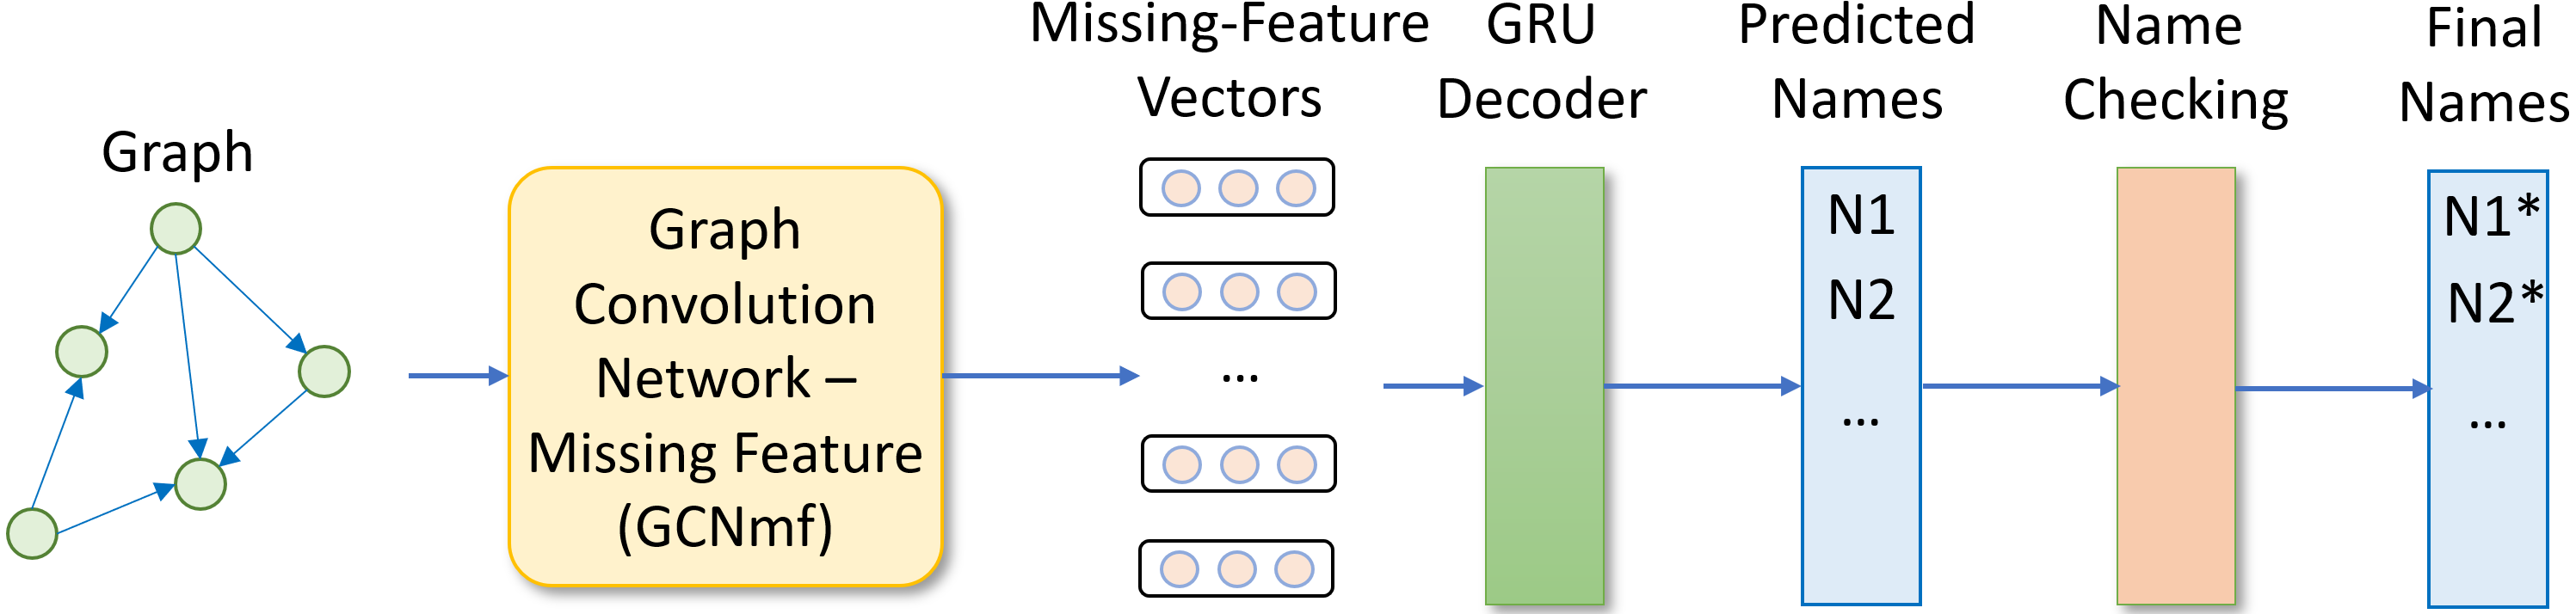
\includegraphics[width=4.8in]{figures/name-gen-model-2}
          \vspace{-6pt}
		\caption{Variables Name Generation Model (VNG)}
		\label{fig:name-gen}
	\end{center}
\end{figure*}


This section presents the Variable Name Generation Model (VNG).
During training, the input is the minified code with all the original
variables' names and types, and during predicting, the input does not
have names and types. First, we build the TDG and the RG for the given
minified code. The two graphs are combined into a representation
graph $G$. For each node in $G$, we tokenize the names in the
corresponding code sequence of the node. We consider each of them as a
sentence and use an embedding model (e.g.,
GloVe~\cite{pennington2014glove}) to build the representation vector
for each node in $G$.

Next, for training, we process the graph $G$ with the node vectors as
follows. For the node $n$ that represents a variable with minified
name, we perform masking the node feature with a special mask token
for the variable name and consider it as a missing feature. Unlike the
VTG model, the VNG model leverages an advanced neural network called
Graph Convolution Network - Missing Features (GCNmf)~\cite{GCNmf}.
The actual names are used as the ground truth labels to train the
GCNmf model. The key characteristic of GCNmf is its ability to deal
with incomplete and missing features in a GCN. It represents the
missing data by Gaussian Mixture Model (GMM) and calculates the
expected activation of neurons in the first hidden layer of GCN, while
keeping the other GCN layers unchanged. The GMM parameters and GCNmf
weight parameters are learned within the same architecture, enabling
the learning of missing features. The GCNmf model is trained with the
masks for the minified variable names. For prediction, applying on the
minified code (without names), the GCMmf model outputs the vectors for
the nodes in the graph $G$ and the vectors for the missing features.

The vectors representing the missing features, i.e., the missing
variables' names in the input graph $G$ are used next to be fed into a
GRU decoder as in the VTG model (Figure~\ref{fig:name-gen}). The
decoder accepts the vectors for missing names as input and generates
the names for the variable nodes (During training, the name labels are
known and used). Finally, we apply the semantic checkers to make sure
that the variables' names are valid in the scope and that the same
variable is assigned with a consistent name.

We use Figure~\ref{rel-graph} as an example to explain how our
variable name generation model works. Because when we use different
code minification tools to process the same source code, the minified
variable names could be different. In this case, the minified variable
names do not have fixed meanings in different codes with varying
minification tools. So in our variable name generation model, when the
generated combined graph comes in, we regard the node $n_r, n_q, n_d$
with the minified variable names such as $r, q, d$ in
Figure~\ref{rel-graph} as the nodes with missing node features. After
feeding the graph into the GCNmf model, it will randomly create
representation vectors $v_r, v_q, v_d$ for nodes $n_r, n_q, n_d$ at
first. During the convolution process, the representation vectors
$v_r, v_q, v_d$ will be automatically updated based on the neighbor
node features and the connection relationships. When the convolution
process is finished, the final stage of representation vectors $v'_r,
v'_q, v'_d$ for nodes $n_r, n_q, n_d$ are fed into the GRU decoder to
predict minified variable names. At the same time, the final
representation vectors for each node can be used in the type
generation model for the type prediction.


Next, let us present the variable name generation model, and then
the dual-task learning between VNG and VTG models.

%1> Similar to step 2, we use GloVe to learn the representation vector.

%2> For the node that represent the variable with minified name, we mask the node feature and regard it as the missing feature.

%3> Put the graph with missing feature for some nodes into the $GCN_{mf}$ as input. 

%4> The $GCN_{mf}$ can output the predicted missing node feature representation vector $V_{rm}$ and the node representation vector $V'_r$. The node representation vector $V'_r$ will be used in step 2.

%5> Use $V_{rm}$ as the input of a GRU (RNN) decoder, and the decoder generate the names for the variables with the minified name.

%6> When doing generation, we apply basic checking to make sure the same variable has only one consistent name.


%Multi-task learning

%We use the uncertainty weighted multi-task loss as the multitask learning loss function and use the maximum of the top-1 accuracy score from two tasks as the training target.
